\documentclass{article}

% if you need to pass options to natbib, use, e.g.:
% \PassOptionsToPackage{numbers, compress}{natbib}
% before loading nips_2017
%
% to avoid loading the natbib package, add option nonatbib:
% \usepackage[nonatbib]{nips_2017}

%\usepackage{nips_2017}

% to compile a camera-ready version, add the [final] option, e.g.:
\PassOptionsToPackage{square, sort, comma, numbers}{natbib}
\usepackage[final]{nips_2017}

\usepackage{amsmath}
\usepackage[utf8]{inputenc} % allow utf-8 input
\usepackage[T1]{fontenc}    % use 8-bit T1 fonts
\usepackage{hyperref}       % hyperlinks
\usepackage{url}            % simple URL typesetting
\usepackage{booktabs}       % professional-quality tables
\usepackage{amsfonts}       % blackboard math symbols
\usepackage{nicefrac}       % compact symbols for 1/2, etc.
\usepackage{microtype}      % microtypography
\usepackage{graphicx}

\title{Linear Multi-step Units: A Worthy Improvement?}

\author{
  Logan Lembke \\
  Department of Computer Science\\
  South Dakota School of Mines and Technology\\
  Rapid City, SD 57701 \\
  \texttt{logan.lembke@mines.sdsmt.edu} \\
}

\begin{document}
% \nipsfinalcopy is no longer used

\maketitle

\begin{abstract}
  In an attempt to provide guidance in the field of neural network design,
  \citet{Lu} presented a new neural network structure, the linear multi-step unit. 
  The linear multi-step unit (LM unit) adapts the common residual unit to one which
  incorporates not only the output of the previous unit, but also the output of
  the unit twice before it. \citet{Lu} claims that networks built from LM units outperform
  similar networks built from residual units when classifying the CIFAR-10 dataset.
  We test these claims and show that while LM units tend to perform better than
  residual units, the benefits are not clear-cut.
\end{abstract}

\section{Introduction}

Underpinning the recent success of several neural network architectures, ResNets \cite{He} allow
neural network practitioners to build deep models with thousands of layers. While ResNets
and their derivatives have proven successful, a guiding framework for the design of neural
network architectures has remained elusive. To this end, \citet{Lu} draws connections between 
differential equation solvers and modern neural network architectures. In particular, 
Lu et al. draws attention to the resemblance between the residual unit which makes up a 
traditional ResNet, and a step of the forward Euler discretization 
$u_{n+1} = u_n + \Delta t f(u_n, t_n)$. Removing $f$'s dependency on $t_n$ and letting 
$\Delta t = 1$ yields $u_{n+1} = u_n + f(u_n)$ which precisely matches the structure of 
a residual unit. 

The forward Euler discretization is one method within the class of linear multi-step methods
for solving ordinary differential equations. Linear multi-step methods use a linear
combination of previous values and derivatives. Additionally, they become more accurate as they
incorporate more terms. \citet{Lu} proposes a neural network structure to match the linear multi-step
discretization given by $u_{n+1} = (1 - k_n)u_n + k_n u_{n-1} + f(u_n) \mid k_n \in \mathbb{R}$, 
called the linear multi-step unit. 

\section{Implementing LM-ResNets}
Applying the linear multi-step unit to a ResNet yields a new network (LM-ResNet) with $N$ more 
parameters where $N$ is the number of residual units. The number of residual units in a ResNet
may be calculated as a function of the number of linear layers, $L$, within the network
$N(L) = (L - 2) / 3$. As such, LM-ResNets require a linear amount of additional weights over 
their standard counterparts as the depth of the network grows.

While \citet{Lu} describe the process by which a ResNet is transformed into a LM-ResNet, several key
details are absent from the description. While a residual unit requires the output from the previous unit, a linear multi-step unit requires the output from the previous two. A traditional ResNet solves this dependency problem by starting out the network with a single convolutional layer. After this first convolutional layer, residual units chain to form the bulk of the network. However, Lu et al. fails to address this issue with regard to LM-ResNets. Several possibilities exist when starting off an LM-ResNet. A single convolutional layer may be used to start the network as in ResNets. This single layer would serve as both $u_n$ and $u_{n-1}$ for the first linear multi-step unit. Alternatively, two convolutional layers may be used to start the network. The outputs of these two layers would serve as $u_n$ and $u_{n-1}$ respectively. As $(1 - k_n)u_n + k_n u_{n-1}$ applies a moving average when $k_n < 1$, we felt justified in using a single convolutional layer in our implementation of LM-ResNets.

\begin{figure}[h]
  \centering
  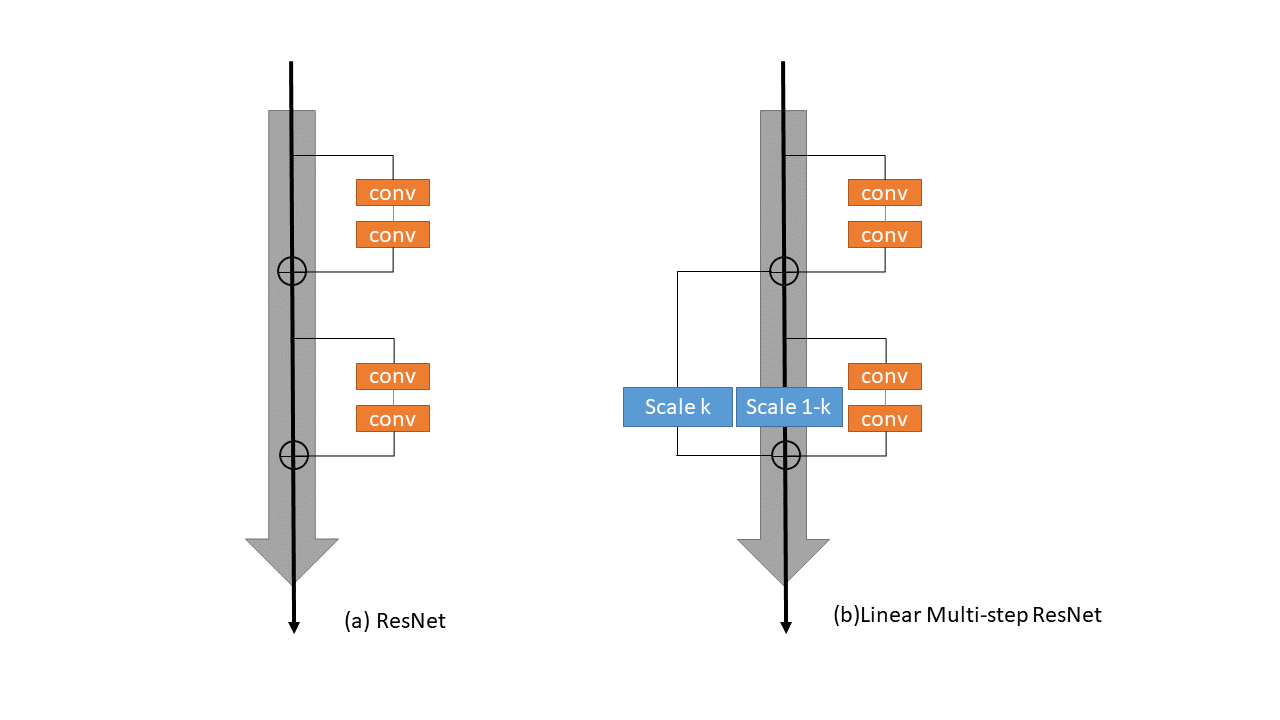
\includegraphics[scale=0.25]{Lu/units.png}
  \caption{(a) Two residual units. (b) One Linear Multi-step residual unit}
\end{figure}

Additionally, \citet{Lu} fails to describe the process by which the projection shortcuts present in
traditional ResNets may be adapted to LM-ResNets. The resolution of the network is cut by strided
convolution at several points in the traditional ResNet architecture. As the shapes of the tensors
being passed through the network change at these layers, a projection shortcut in the form of a 1x1 strided convolution is introduced in place of the identity connection to facilitate addition. This projection shortcut uses a separate set of weights from the strided convolution in 
the $f(x)$ unit. $u_{n+1} = u_n + f(u_n)$ becomes $u_{n+1} = proj(u_n) + f(u_n)$. 

In a LM-ResNet, one or both of $u_n$ and $u_{n-1}$ may be of inappropriate shape to add to $f(u_n)$. 
$u_{n+1} = (1 - k_n)u_n + k_n u_{n-1} + f(u_n)$ becomes $u_{n+1} = (1 - k_n)proj(u_n) + k_n proj(u_{n-1}) + f(u_n)$. As this projection serves to transform the data into a lower dimensional
space from a space shared by both $u_n$ and $u_{n-1}$, we elected to implement weight sharing for each
projection shortcut in the original ResNet. 

\section{LM-ResNets vs ResNets}

\citet{Lu} claims that LM-ResNets significantly outperform traditional ResNets on the CIFAR-10 dataset.
We tested this claim by building a reference implementation of LM-ResNets based on the official
Tensorflow ResNet implementation. Hyperparameters were adjusted to meet the specifications in \citep{Lu}.
Parameters $k_n$ were initialized using a uniform distribution between $-0.1$ and $0$.
\begin{table}[h]
  \caption{Hyperparameters}
  \centering
  \begin{tabular}{ll}
    \toprule
    Parameter             & Value     \\
    \midrule
    Training Epochs       & 160       \\
    Batch Size            & 128       \\
    Weight Decay          & 0.0001    \\
    Momentum              & 0.9       \\
    Initial Learning Rate & 0.1       \\
    Learning Rate Decay   & 0.1, 0.01 \\
    LR Decay Epochs 	  & 80, 120   \\
    \bottomrule
  \end{tabular}
\end{table}

Additionally, data augmentation was carried out in accordance with the practices in \citet{Lu} and \citet{He}.
Each image was randomly, horizontally flipped, padded with four on pixels each side, cropped back down
to 32x32, and normalized. 

Both ResNets and LM-ResNets were trained at various depths including 20, 32, 44, 56, and 110 linear layers. 
All of the networks trained in roughly the same fashion. The biggest drops in the loss occurred
when the learning rate decay took place. 

\begin{figure}[h]
  \centering    
  \def\svgwidth{\columnwidth}
  \input{train_loss/resnet.pdf_tex}
  \caption{ResNet training losses using various amounts of layers}
\end{figure}

\begin{figure}[h]
  \centering    
  \def\svgwidth{\columnwidth}
  \input{train_loss/lmnet.pdf_tex}
  \caption{LM-ResNet training losses using various amounts of layers}
\end{figure}

After 160 epochs of training, the test accuracies of each network were compared. 
For all but the 20 and 110 layer network, LM-ResNets eked out slightly higher 
accuracies with improvements on the order of thousandths of percentiles. However,
the ResNet implementation won out when using very shallow and very deep networks.

\begin{table}[!ht]
  \caption{Test Accuracy after 160 Epochs}
  \centering
  \begin{tabular}{lllll}
    \toprule
    Depth & ResNet (ours) & LM-ResNet (ours) & ResNet (theirs) & LM-ResNet (theirs) \\
    \midrule
    20    & .9142 & .9121 & .9125 & .9167\\
    32    & .9179 & .9197 & .9249 & .9282\\
    44    & .9228 & .9233 & .9283 & .9334\\
    56    & .9244 & .9269 & .9303 & .9369\\
    110   & .9294 & .9286 & .9363 & Not Reported\\
    \bottomrule
  \end{tabular}
\end{table}

\begin{figure}[!ht]
  \centering    
  \def\svgwidth{\columnwidth}
  \input{test_accuracy/resnet.pdf_tex}
  \caption{ResNet test accuracy using various amounts of layers}
\end{figure}

\begin{figure}[!ht]
  \centering    
  \def\svgwidth{\columnwidth}
  \input{test_accuracy/lmnet.pdf_tex}
  \caption{LM-ResNet test accuracy using various amounts of layers}
\end{figure}

However, due to the stochastic nature of training, it may be unfair to compare
test accuracy at the end of training. For this reason, we compare each ResNet
against its respective LM-ResNet at each depth. During the first phase of 
training (learning rate = 0.1), comparisons are made difficult by the correspondingly large
movements in accuracy. Once the learning rate decreases to 0.01, the LM-ResNets
take the lead across the board. However, once the learning rate decreases 
to its final value, 0.001, ResNets narrow in on the gap, and in the case of the 
20 and 110 layer networks, the ResNets overtake the LM-ResNets. 
 
\begin{figure}[!t]
  \centering    
  \def\svgwidth{\columnwidth}
  \input{test_accuracy/cmp_20.pdf_tex}
  \caption{Test accuracies over time for a LM-ResNet and ResNet using 20 layers}
  \def\svgwidth{\columnwidth}
  \input{test_accuracy/cmp_32.pdf_tex}
  \caption{Test accuracies over time for a LM-ResNet and ResNet using 32 layers}
  \def\svgwidth{\columnwidth}
  \input{test_accuracy/cmp_44.pdf_tex}
  \caption{Test accuracies over time for a LM-ResNet and ResNet using 44 layers}
\end{figure}

\begin{figure}[!ht]
  \centering    
  \def\svgwidth{\columnwidth}
  \input{test_accuracy/cmp_56.pdf_tex}
  \caption{Test accuracies over time for a LM-ResNet and ResNet using 56 layers}
\end{figure}

\begin{figure}[!ht]
  \centering    
  \def\svgwidth{\columnwidth}
  \input{test_accuracy/cmp_110.pdf_tex}
  \caption{Test accuracies over time for a LM-ResNet and ResNet using 110 layers}
\end{figure}

\vbox{
\section{Conclusions}
In our testing, LM-ResNets offer improvements on the order of thousandths of percentiles over traditional ResNets.
However, they sometimes perform worse, especially on extremely shallow or deep networks. We did not see the 
consistent improvements claimed by \citet{Lu}. However, several factors may contribute to this discrepancy. 

First, we only ran one instance of each network. As training neural networks incorporates non-deterministic 
algorithms, a sample of runs aught to be taken for each comparison. Perhaps it was chance that the LM-ResNets
performed as poorly as they did. 
}
Second, the official CIFAR-10 ResNet accuracies are consistently higher than our own. Our implementation stemmed
from the official Tensorflow implementation. Several other Tensorflow users haver reported similar performance
problems with the official implementation. However, the high level code has been reviewed by several authors
and found to be correct. Implementations in other frameworks do not appear to have this issue.

Finally, several implementation details were missing from the description of LM units. In order to avoid adding
additional parameters to our model, we implemented our LM-ResNets using a single convolutional layer at the
beginning, and one set of convolutional weights each time a projection shortcut was needed. Using two convolutional layers at the beginning, or creating separate weights for each projection operation would increase the 
representational capacity of the network and may increase test accuracy. 

Future research may cover implementing more skip connections including more data from previous layers. Connections
with the DenseNet architecture may be made to ODE solvers and the linear multi-step architecture. Additionally,
the parameterization of the addition step may be investigated. Explicitly modeling the free parameter as time with
the Adams-Bashforth linear multi-step method may provide interesting results.

\bibliographystyle{plainnat}
\bibliography{ml}


\end{document}
